\label{chapter-3}
Data extraction and indexing from various blockchains is an essential topic for making Web3 and dApps working, there are different projects that have tried to address this problem. A lot of work has been done by companies, whose source code and methodology are not publicly available. There are also some open source or academic attempts that I use as a comparison with my work. \\

\noindent These projects target three main categories:

\begin{itemize}
  \item Web3 and dApps developers, that need data to feed their applications.
  \item Data analysts, that need to analyse historical blockchain data. 
  \item Blockchain users, that need to see the results of transactions.
\end{itemize}

\noindent In the next sections I list the state of the art tools available.

\section{Etherscan}

In the world of blockchain, \textit{explorers} play an important role. They are web-based tools that allow users to see every kind of information with a user-friendly and interactive interface.

Etherscan\footnote{Online blockchain explorer available at \url{https://etherscan.io/}} is the reference point for accessing data about the Ethereum blockchain. It is the most used Ethereum explorer that lets people browse historical data through a web interface. Here users can easily explore transactions, internal calls, token transfers and everything else related to the Ethereum protocol. It is useful for inspecting singular operations, but it can not be used for large-scale analysis.

One of the most important services they offer is the verification of smart contracts, they host 461,261\footnote{This data was calculated using the CSV file exported from \url{https://etherscan.io/chart/verified-contracts}} source codes (as of 17 May 2023) that have been verified to match exactly the deployed bytecode on the Ethereum chain. 

The process of verification consists in providing Etherscan the exact source code of a Smart Contract, the version of the compiler used, the license selected and the contract address to verify. With this information, Etherscan tries to compile the given data and check if the resulting bytecode equals the one deployed on the blockchain. If the check succeeds, then the source code correctly describes the bytecode of the smart contract. There are plugins for the most used development tools like Remix\footnote{Remix is an online IDE to develop Ethereum smart contracts. It is possible to verify contracts using the {\it Etherscan Contract Verification} plugin. A detailed guide can be found here: \url{https://medium.com/@ezeamaka2/how-to-verify-smart-contracts-on-etherscan-in-remix-ide-92f6354933b4}.} or Hardhat\footnote{Hardhat is a popular Ethereum development environment. It has the \textit{hardhat-verify} plugin that allows to verify contracts easily: \url{https://hardhat.org/hardhat-runner/plugins/nomicfoundation-hardhat-verify}.} that ease this process of verification.

This data is helpful for understanding the semantics of the code deployed, since it is hard to get valuable insights by just looking at the raw bytecode. Many studies are based on these verified contracts.

Etherscan has evolved from being just an Ethereum explorer. Etherscan developers use the Ethereum blockchain data and created API endpoints and offer these data to users for a fee. These API endpoints include the standard Ethereum JSON-RPC interface. There are also other more advanced indexes not supported by the standard RPC, e.g.~transactions by address, ABI of contracts, token transfers.

On top of that, they also provide live and interactive charts\footnote{Interactive charts are available at \url{https://etherscan.io/charts}} about historical Ethereum data.

The same company that is behind the Ethereum Etherscan explorer applied the same logic and technology to other EVM-compatible chains, like Polygon\footnote{Explorer for the Polygon network \url{https://polygonscan.com/}} or BNB Smart Chain\footnote{Explorer for the BNB Smart Chain \url{https://bscscan.com/}}.

It is important to note that, although they provide almost all the possible available Ethereum data, they have not shared technical details about how this data is extracted or how it is indexed. Users need to trust the company. Another problem is that the data they offer is not easy to get and manipulate for large-scale analysis. Their API service is meant to be used by developers for building dApps. It would be too expensive to use it for data analysis on all the history of the chain. 

\section{The Graph}

The Graph~\cite{the-graph} is a decentralized indexing protocol for blockchain data. It allows users to get structured on-chain data from other users via a GraphQL\footnote{GraphQL is an open source query language managed by Linux Foundation, originally created by Facebook.} interface. 

All the data is organized in so-called \textbf{subgraphs}, which are independent data collections that index a small subset of a blockchain network. A common pattern is that a subgraph indexes data from one or a set of few smart contracts all part of a common protocol, like Uniswap\footnote{Uniswap is a decentralized cryptocurrency exchange \url{https://uniswap.org/}}. All the available subgraphs can be found on the \textit{Graph Explorer}\footnote{The Graph Explorer collects all the subgraphs of the protocol, it is available at: \url{https://thegraph.com/explorer}}.

The underlying protocol is composed of multiple actors:

\begin{itemize}
  \item Developers: people with technical knowledge that develop the needed code for creating and maintaining the indexes. As of now, the most important pieces of code needed are the mappings from Ethereum events to the stored data, written in AssemblyScript\footnote{AssemblyScript is a Typescript-like language that is compiled to WebAssembly.}, and the subgraph manifest, a structured description of all the parts needed by the subgraph in YAML format.  
  \item Indexers: they are responsible for operating a node. This implies indexing the data following a subgraph specification and serving queries to users.
  \item Curators: they are in charge of finding the best subgraphs to be indexed.
  \item Delegators: they secure the network by locking economical value to certain indexers they choose, giving them the possibility to serve more queries.
\end{itemize}

\begin{figure}[!ht]
  \centering
  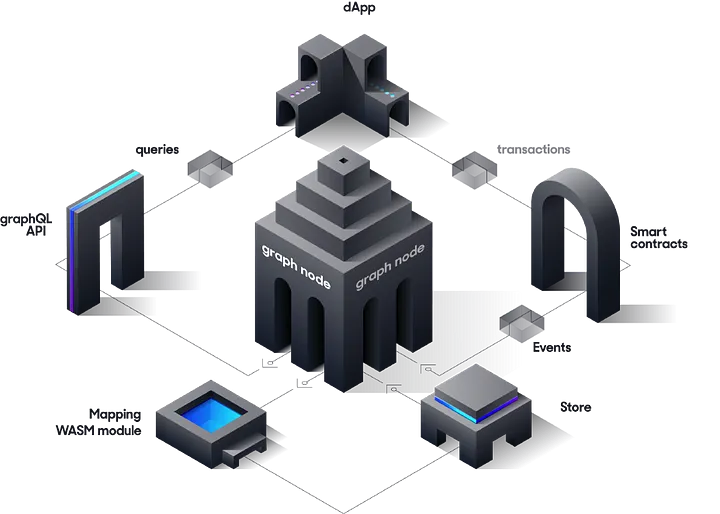
\includegraphics[width=1\textwidth]{Figures/graph-dataflow.png}
  \caption[The Graph data flow]{Data flow of The Graph indexing protocol\protect\footnotemark.}
  \label{fig:the-graph-data-flow}
\end{figure}

\footnotetext{Source: \url{https://thegraph.com/docs/en/about/}}

All these actors are economically motivated to perform well. This is achieved via a token economy where the GRT is the currency. It is implemented on the Ethereum chain with an ERC-20 smart contract\footnote{\url{https://etherscan.io/token/0xc944e90c64b2c07662a292be6244bdf05cda44a7}}.

In order to index and serve queries, indexers have to stake at least 100,000 GRT tokens (roughly equal to 12K USD with the current change). These tokens can be slashed in case the indexer behaves maliciously. The more tokens the indexer stakes and the more queries it can serve. At the same time, indexers are rewarded with GRT tokens in two ways: query fees and annual rewards based on amount of queries served.

According to the specification of the subgraph file\footnote{Specification available at: \url{https://github.com/graphprotocol/graph-node/blob/master/docs/subgraph-manifest.md\#15-data-source}}, the only allowed source of data are Ethereum contracts and mappings are restricted to logs. \Cref{fig:the-graph-data-flow} shows the flow of data in the protocol. In most cases, this is enough for dApps, since typically all the smart contracts are written in such a way that they emit meaningful events when things happen. 

On the other hand, it is not possible to index all the other kind of information for performing other analysis, such as block data, contract deployments, transactions, contracts destruction, etc. It is also not possible to extract data that was not meant to be extracted, since the emitted events are pieces of information that the developers of the smart contracts explicitly wanted to expose and index. 

As of today, the protocol continues to rely on a centrally hosted service that uses the subgraphs' logic and code to index data, but queries are served from this centralized server for free. This should change later in 2023, the network should slowly migrate from this centralized service to the decentralized protocol once the quality of the service will be comparable\footnote{This transition is explained in details here: \url{https://thegraph.academy/developers/sunsetting-the-hosted-service/}}.

The Graph is the first attempt to decentralize indexing of blockchain data, it is still a project with a lot of work behind the scene. It is the most promising mechanism to make Web3 and dApps not dependent on centralized data ingestion services.

\section{Ethereum-ETL}

Ethereum-ETL~\cite{ethereum-etl}~is an open-source tool for extracting data from the Ethereum blockchain following the \textbf{Extract-Transform-Load} pattern. It is written in Python and can be used through a CLI.

\noindent Raw data can be extracted to CSV or JSON files using these commands:

\begin{itemize}
    \item \verb|export_blocks_and_transactions|: it calls \verb|eth_getBlockByNumber| RPC and maps the response to two files containing blocks and transactions.
    \item \verb|export_token_transfers|: it calls \verb|eth_getFilterlogs| applying a filter with the first topic set to the Keccak-256 hash of the Transfer event signature. Transfers are stored in a single file without distinction between ERC20 or ERC721.   
    \item \verb|export_traces|: it stores the internal transactions calling the \verb|trace_block| method.
\end{itemize}

\noindent All other kind of data can be extracted starting from the files that these previous commands store. It is possible to further extract:

\begin{itemize}
    \item Transaction receipts and logs starting from transaction hashes exported from \verb|export_blocks_and_transactions|.
    \item Contracts data, starting from the traces stored with \verb|export_traces|.
    \item Token contracts with metadata, starting from contracts (this requires two previous steps of extraction). 
\end{itemize}

Ethereum-ETL also provides the command {\tt export\_all} to perform extraction of all the common data in a single step (blocks, transactions, receipts, logs, contracts, token transfers and token metadata). However, this command is not present in the documentation and it can not extract contracts deployed by other contracts, just the ones deployed by Externally Owned Accounts. 

\subsection{Google BigQuery public dataset}

\noindent Ethereum-ETL also allows for streaming data from an Ethereum node to the console. This functionality is used to ingest data into the popular Ethereum Google BigQuery public dataset\footnote{The Google's BigQuery dtaset can be explored here: \url{https://cloud.google.com/blog/products/data-analytics/ethereum-bigquery-public-dataset-smart-contract-analytics}}. This dataset is organized in six tables that I report here in \cref{table:bigquery-blocks,table:bigquery-contracts,table:bigquery-logs,table:bigquery-traces,table:bigquery-transactions,table:bigquery-transfers} since it is a good representation of the raw data that can be extracted from an Ethereum node.

\begin{table}[H]
\centering
    \begin{tabular}  { m{6cm} m{3cm} m{3cm} } 
    \toprule
    \textbf{Attribute} & \textbf{Type} & \textbf{Required} \\
    \midrule
    timestamp & Timestamp & Yes\\ %& The timestamp for when the block was collated	\\
    number & Integer & Yes\\ %& & The block number \\
    hash & String & Yes\\ %& & Hash of the block \\
    parent\_hash & String & No\\ %& & Hash of the parent block\\
    nonce & String & Yes\\ %& Hash of the generated proof-of-work \\
    sha3\_uncles & String & No\\ %& & SHA3 of the uncles data in the block \\
    logs\_bloom & String & No\\ %& & The bloom filter for the logs of the block \\
    transaction\_root & String & No\\ %& & The root of the transaction trie of the block \\
    state\_root& String & No\\ %& & The root of the final state trie of the block \\
    receipt\_root & String & No\\ %& & The root of the receipts trie of the block \\
    miner & String & No\\ %& & The address of the beneficiary to whom the mining rewards were given \\
    difficulty & Numeric & No\\ %& & Integer of the difficulty for this block\\
    total\_difficulty & Numeric & No\\ %& & Integer of the total difficulty of the chain until this block\\
    size & Integer & No\\ %& & The size of this block in bytes\\
    extra\_data & String & No\\ %& & The extra data field of this block\\
    gas\_limit & Integer & No\\ %& & The maximum gas allowed in this block\\
    gas\_used & Integer & No\\ %& & The total used gas by all transactions in this block \\
    transaction\_count & Integer & No\\ %& & The number of transactions in the block \\
    base\_fee\_per\_gas & Integer & No\\ %& & Protocol base fee per gas, which can move up or down \\
    withdrawals\_root & String & No\\ %& & The root of the withdrawal trie of the block\\
    withdrawals & Record & Repeated\\ %& & Validator withdrawals \\
    \quad- index & \quad- Integer & \quad- No\\ %& &  \\
    \quad- validator\_index & \quad- Integer & \quad- No\\ %& & \\
    \quad- address & \quad- Integer & \quad- No\\ %& & \\
    \quad- amount & \quad- Integer & \quad- No\\ %& & \\
    \bottomrule
\end{tabular}
\caption[Google BigQuery \texttt{Blocks} table]{Schema of table \textit{Blocks} on the Google BigQuery public dataset. Taken from the official docs.}
\label{table:bigquery-blocks}
\end{table}

\begin{table}[H]
\centering
    \begin{tabular}  { m{6cm} m{3cm} m{3cm} } 
    \toprule
    \textbf{Attribute} & \textbf{Type} & \textbf{Required} \\
    \midrule
    log\_index & Integer	& Yes \\
    transaction\_hash & String & Yes \\
    transaction\_index & Integer & Yes	\\		
    address & String & No \\
    data & String & No \\
    topics & String & Repeated \\
    block\_timestamp & Timestamp & Yes \\ 
    block\_number & Integer & Yes \\
    block\_hash & String & Yes \\
    \bottomrule
\end{tabular}
\caption[Google BigQuery \texttt{Logs} table]{Schema of table \textit{Logs} on the Google BigQuery public dataset. Taken from the official docs.}
\label{table:bigquery-logs}
\end{table}

\begin{table}[H]
\centering
    \begin{tabular}  { m{6cm} m{3cm} m{3cm} } 
    \toprule
    \textbf{Attribute} & \textbf{Type} & \textbf{Required} \\
    \midrule
    address & String & Yes \\
    bytecode & String & No \\
    function\_signature & String & repeated \\
    is\_erc20 & Boolean & No \\
    is\_erc721 & Boolean & No \\
    block\_timestamp & Timestamp & Yes \\
    block\_number & Integer & Yes \\
    block\_hash & String & Yes \\
    \bottomrule
\end{tabular}
\caption[Google BigQuery \texttt{Contracts} table]{Schema of table \textit{Contracts} on the Google BigQuery public dataset. Taken from the official docs.}
\label{table:bigquery-contracts}
\end{table}

\begin{table}[H]
\centering
    \begin{tabular}  { m{6cm} m{3cm} m{3cm} } 
    \toprule
    \textbf{Attribute} & \textbf{Type} & \textbf{Required} \\
    \midrule
    transaction\_hash & String &	No	\\			
    transaction\_index & Integer	& No	\\			
    from\_address & String &	No \\	
    to\_address & String & No \\				
    value & Numeric &	No		\\		
    input & String &	No		\\		
    output & String	& No		\\		
    trace\_type & String &	Yes		\\		
    call\_type & String	& No	\\
    reward\_type & String	& No\\
    gas & Integer	& No\\
    gas\_used & Integer	& No\\
    subtraces & Integer	& No\\
    trace\_address & String	& No		\\
    error & String	& No		\\
    status & Integer	& No	\\		
    block\_timestamp & Timestamp	& Yes		\\		
    block\_number & Integer	& Yes			\\	
    block\_hash & String	& Yes	\\			
    trace\_id & String	& No \\
    \bottomrule
\end{tabular}
\caption[Google BigQuery \texttt{Traces} table]{Schema of the \textit{Traces} table on the Google BigQuery public dataset. Taken from the official docs.}
\label{table:bigquery-traces}
\end{table}

\begin{table}[H]
\centering
    \begin{tabular}  { m{6cm} m{3cm} m{3cm} } 
    \toprule
    \textbf{Attribute} & \textbf{Type} & \textbf{Required} \\
    \midrule
    token\_address & String & Yes	 \\			
    from\_address & String & No \\
    to\_address & String	& No	\\			
    value & String	& No	\\
    \bottomrule
\end{tabular}
\caption[Google BigQuery \texttt{Token\_transfers} table]{Schema of table \textit{Token\_transfers} on the Google BigQuery public dataset. Taken from the official docs.}
\label{table:bigquery-transfers}
\end{table}

\begin{table}[H]
\centering
    \begin{tabular}  { m{6cm} m{3cm} m{3cm} } 
    \toprule
    \textbf{Attribute} & \textbf{Type} & \textbf{Required} \\
    \midrule
    hash & String	& Yes		\\		
    nonce & Integer	& Yes \\				
    transaction\_index & Integer	& Yes		\\		
    from\_address & String	& Yes			\\	
    to\_address & String	& No		\\		
    value & Numeric	& No \\				
    gas &  Integer	& No \\				 
    gas\_price &  Integer &	No \\				
    input &  String	& No \\				
    receipt\_cumulative\_gas\_used & Integer & 	No \\				
    receipt\_gas\_used  & Integer	& No \\				
    receipt\_contract\_address & String	& No \\				
    receipt\_root &  String & 	No \\				
    receipt\_status  & Integer & 	No \\				
    block\_timestamp  & Timestamp	 & Yes \\				
    block\_number  & Integer & 	Yes \\				
    block\_hash & String &	Yes \\				
    max\_fee\_per\_gas & Integer	& No \\	
    max\_priority\_fee\_per\_gas & Integer	& No \\		
    transaction\_type & Integer	& No				\\
    receipt\_effective\_gas\_price & Integer	& No	\\
    \bottomrule
\end{tabular}
\caption[Google BigQuery \texttt{Transactions} table]{Schema of table \textit{Transactions} on the Google BigQuery public dataset. Taken from the official docs.}
\label{table:bigquery-transactions}
\end{table}

It is possible to query these tables using SQL syntax, they can be joined on equal fields. There is the possibility to query this database for free up to a certain monthly limit of processing storage and amount of data extracted. 

\section{Dune Analytics}

Dune Analytics\footnote{Blockchain analytics platform \url{https://dune.com/home}} is a company that provides tools to query and visualize data from multiple blockchains. They support Bitcoin, Solana, Ethereum and other 8 EVM-compatible chains.\\

Their application is web-based. With their web-app it is possible to create queries using SQL syntax and visualize results in interactive charts. Multiple queries can be collected together to create dashboards\footnote{Example of a dashboard about history of Ethereum: \url{https://dune.com/hildobby/ethereum}}.  

\subsection{Data architecture}

Blockchain data was initially managed using PostgreSQL and SparkSQL until 2022, year in which they released their own engine called DuneSQL \footnote{DuneSQL was announced in this blog post: \url{https://dune.com/blog/dune-engine-v2}}. The migration to this technology is currently ongoing. \\

They started storing and indexing data with PostgreSQL.
In this DBMS, entries are stored in pages following a row-oriented strategy, which means that all the attributes of a row are stored adjacently. 
This strategy is beneficial when it is necessary to retrieve all the attributes of a row while querying. 
However, it leads to poor performances when filtering for specific attributes, since the database has to load many bytes containing irrelevant data (i.e., all the other attributes of the row that are not used). 
To avoid this, it is possible to create indexes on columns. 
Indexes avoid the need to read and filter data. They provide direct access to the location of the requested data.
Indexes provide very good query performances, but can be hard and slow to maintain when the amount of data grows.
At Dune Analytics they tried this approach with traditional relational database (PostgreSQL) combined with many indexes, but they had to drop it stating that "the size of the datasets were so huge that the database was struggling to fully support them"\footnote{Source: \url{https://dune.com/blog/introducing-dune-sql}}. \\

They came up with DuneSQL, a query engine built specifically for managing blockchain data. It is a fork of Trino, an open source distributed SQL query engine designed to query data from heterogeneous sources. The DuneSQL fork is not open-source, so technical information can only be deducted from their blog articles or statements on the support community. The main features they added are \textit{varbinary} data type for storing addresses and hashes, as well as \textit{uint256} support for EVM data. \\

Data is physically stored on AWS S3 buckets using the Apache Parquet storage format\footnote{Detailed description of Parquet storage format \url{https://github.com/apache/parquet-format}}. This storage system is a mix between column and row oriented. Data is split in files based on rows, inside these files, there are further row groups and inside these groups data is divided by columns. \cref{fig:parquet-structure} visualizes this concept. 

\begin{lstlisting}[language=SQL,caption={Shortened simple query on DuneSQL that took 3 minutes to run},label={lst:dune-query},captionpos=b]
Select * from ethereum.transactions
where hash = 0x9ef65fe51...ff74219e
\end{lstlisting}

Indexing is done using the Parquet file's metadata. At the end of each file there is a part in which are stored min/max values of all the column values inside a row group, as shown in image \ref{fig:parquet-index}. This information allows the database to skip reading the whole file if values are not in the desired range. While working great for certain types of data, it is not very useful with strings, especially if they are not sorted. That is the reason why even very simple queries can take several minutes to run. \cref{lst:dune-query} serves as an example of such a query. 

\begin{figure}[!ht]
  \centering
  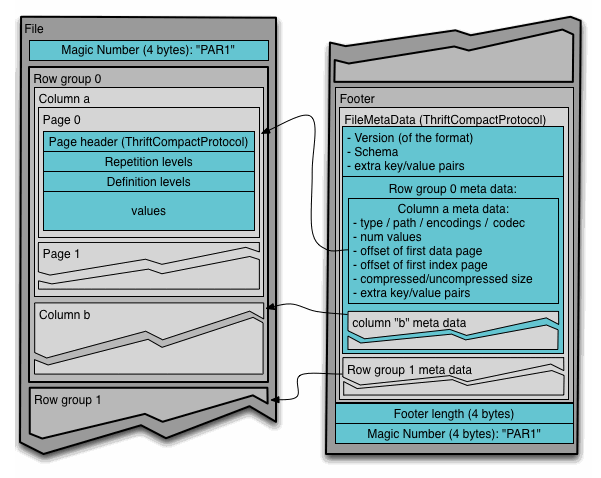
\includegraphics[width=1\textwidth]{Figures/parquet-structure.png}
  \caption[Parquet storage format structure]{File structure in the Parquet storage format\protect\footnotemark.}
  \label{fig:parquet-structure}
\end{figure}

\footnotetext{Source: \url{https://github.com/apache/parquet-format}}

\begin{figure}[!ht]
  \centering
  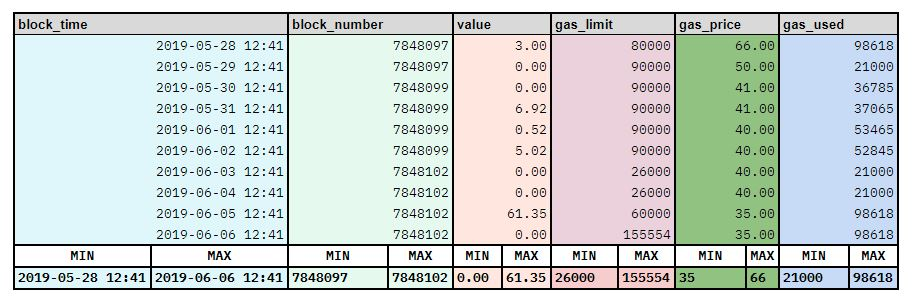
\includegraphics[width=1\textwidth]{Figures/parquet-index.jpg}
  \caption[Parquet ColumnIndex on Dune Analytics]{Parquet min/max column index structure \protect\footnotemark. }
  \label{fig:parquet-index}
\end{figure}

\footnotetext{Source: \url{https://dune.com/docs/query/storage/}}


\subsection{Available data}

On Dune Analytics, blockchain data is available in multiple layers:

\begin{itemize}
    \item \textit{Raw tables}: these tables contain raw data as it is stored on the various blockchains, without modifications. For EVM chains this means Blocks, Logs, Traces, Transactions and Withdrawals.
    \item \textit{Decoded tables}: smart contracts with verified source code receive their own tables on which data is stored in a more readable way. Each event and function that is present in the contract's ABI corresponds to a table on Dune with the following name pattern: \texttt{project\_chain.contract\_[evt/call]\_evtOrCallName}. Inside this table there will be columns for each of the event or function attributes, with the relative names. For example, all the \textit{cryptokitties} \texttt{Transfer} events are stored in a table called \texttt{cryptokitties\_ethereum.KittyCore\_evt\_Transfer} that will have, among other contextual information, three columns: \textit{from}/\textit{to} addresses and \textit{tokenId}.
    \item \textit{Spellbooks}: these tables are abstractions over raw and decoded data that give users an easy way to retrieve information without diving into the technicalities of complex decentralized protocols. They are open source and the community can contribute creating new spellbooks on the Github Repository\footnote{All the spellbooks can be found on the Github repository: \url{https://github.com/duneanalytics/spellbook}}. The main power of spellbooks is to put together data from heterogeneous sources to gather useful insights. One of the clearest example is the \texttt{dex.trades}\footnote{Source code of the \texttt{dex.trades} spellbook: \url{https://github.com/duneanalytics/spellbook/blob/main/models/dex/dex\_trades.sql}} spellbook, that puts together all the trades made on all decentralized exchanges of all the blockchains present on Dune Analytics.
\end{itemize}

\section{XBlock-ETH}

Zheng et al.~\cite{xblock-eth} released a dataset containing raw Ethereum data and described the framework used for getting it, called XBlock-ETH. It was released in 2019. Data is periodically updated in chunks of 500,000 blocks, it currently covers blocks from 0 to 16,499,999. It is divided in different smaller datasets: \textit{Block}, \textit{Block Transaction}, \textit{Internal Transaction}, \textit{Contract Info}, \textit{ERC20 Transaction}, \textit{ERC721 Transaction}, \textit{Token Info}. Data can be downloaded from their website\footnote{Xbloxk website where it is possible to get the data: \url{https://xblock.pro/xblock-eth.html}} in CSV format.

This is a useful resource for getting Ethereum data without having the possibility to run a node; however it lacks important information such as logs and receipts. 

It is not easy to use, since the massive amount of data in the CSV files must be parsed and cannot be easily queried or indexed, further transformation steps are needed. There are some Python scripts available on Github\footnote{Repository of XBlock-ETH: \url{https://github.com/tczpl/XBlock-ETH}} for downloading and analysing the data, but the code used for the extraction is not open-source, so it is not possible to replicate the extraction.

\section{Data-ether}

DateEther \cite{dataether} is a framework presented by Chen et al.~for extracting and indexing Ethereum data. They tried a different approach for executing this task: they modified a Geth node to record and store data during the initial synchronization phase. They used ElasticSearch\footnote{ElasticSearch is a search engine based on the Lucene library \url{https://www.elastic.co/}} for indexing and exploring data, but by the time of their research the size of data was relatively small compared to now.

While extracting data by modifying a node source code was efficient back in 2019, now Ethereum nodes have evolved and there are different and faster RPCs for getting internal transactions. Their way of extracting data was compared against \texttt{debug\_traceTransaction} RPC of Geth, claiming to be 18.6x faster, but it was not compared against \texttt{debug\_traceBlock} or \texttt{trace\_block} of Erigon. From my work, using Erigon's \texttt{trace\_block} RPC, I managed to get and loop trough all the internal transactions in around 7 hours. Doing that while synchronizing a node would have required at least 3-4 days. 

Extracting data by modifying source code has another drawback: maintainability. Just Geth itself received 173 releases\footnote{Data obtained from the Github releases page: \url{https://github.com/ethereum/go-ethereum/releases}}, modifying its source code would mean having to merge the code and resolving eventual conflicts every time a new release is published. This is not a problem using Ethereum RPC APIs since they do not change after upgrades of the nodes.

\section{Web3 providers}

The term \textit{Web3 provider} is commonly used to refer to companies that offer access to Ethereum RPC API, avoiding developers of Web3 dApps the costs of running a node. They are included in this chapter since the majority of them also provide access to more sophisticated indexed and interpreted data. Some popular web3 providers include Alchemy\footnote{\url{https://www.alchemy.com/}}, Infura\footnote{\url{https://www.infura.io/}}, Quicknode\footnote{\url{https://www.quicknode.com/}} and Chainstack\footnote{\url{https://chainstack.com/}}.

All of them have endpoints for getting NFTs data. It is possible to get all NFTs owned by an address by just calling an API instead of having to analyze all the chain. Chainstack also hosts on their servers all the supgraphs of \textit{The Graph} protocol, offering users the possibility to use a more stable service instead of the decentralized alternative.

It is important to note that the web3 providers are profit-oriented companies. While they provide an important service in the world of dApps, it is essential to consider their cost implications. Using their services for analyzing historical data can be very expensive, since billing is done based on number of API requests to their server.

Another important aspect to consider is the transparency of these services. As profit-oriented entities, these web3 providers do not necessarily make their source code and methodology open-source. This means that developers relying on their services need to trust the data they receive. 

Depending on centralized companies poses also a risk to the actual decentralization of the web3. Access to the blockchain infrastructure is concentrated on a few companies, as noted by Wang et al.~\cite{wang2022exploring}.

\section{Comparison}

\cref{table:tools-comparison} summarises the main differences between the analyzed tools in terms of \textit{primary target}, \textit{transparency} and \textit{price}.

\begin{table}[ht!]
\centering
    \begin{threeparttable}
    \begin{tabular}  { m{3cm} m{3cm} m{1.5cm} m{5cm} } 
    \toprule
    \textbf{Tool} & \textbf{Target} & \textbf{Open source} & \textbf{Price}  \\
    \midrule
    Etherscan    & Blockchain users  & No & Free explorer, paid apis  \\[2.3ex]
    The Graph     & Web3 developers & Yes & Billing based on usage  \\[1.3ex]
    Ethereum-ETL     & Data analysts & Yes & Free  \\[1.3ex]
    Dune Analytics      & Data analysts & No & Based on query credits, it has free plan \\[2.6ex]
    XBlock-ETH  & Data analysts & No\tnote{*} & Free   \\[1.3ex]
    DataEther  & Data analysts & No\tnote{*} & Free   \\[1.3ex]
    Web3 providers      & Web3 developers & No & Billing on usage, they have free plans   \\[1.6ex]
    \bottomrule
    \end{tabular}
    \begin{tablenotes}
      \item[*] Source code not available, but technical papers describing the software were released.
      \end{tablenotes}
    \end{threeparttable}
\caption[State of the art tools comparison]{Comparison of state-of-the art tools for management of blockchain data.}
\label{table:tools-comparison}
\end{table}

My work aims to provide an open-source alternative for accessing Ethereum data. The main target are data analysts, but thanks to the performance of the database used, it can also be used by web3 developers. It is mostly inspired by Ethereum-ETL, but with particular focus on performance and semantics of smart contracts. Data is indexed using a particular graph database, Dgraph, that was not used in the other works.
